\chapter{Matching} \label{chapter:matching}
The following chapter presents the parallelization approaches suggested in this work. %These include some of the more ``traditional'' skyline algorithms, such as Naive-Nested-Loops and DNC, as well as two of the newer algorithms ST-S and SARTS. 
All the algorithms were implemented and parallelized in C++, mainly due to its efficiency in terms of speed and memory management. 

\section{Methods and Frameworks} \label{section:methods-frameworks}
There are two different implementation models used for the algorithms. The Block-Nested-Loops algorithm is implemented in two versions: one of them makes use of the Volcano model, the other of the produce/consume concept. This was done in order to be able to compare the two models in terms of their performance. The rest of the algorithms were implemented with the produce/consume concept only. Both models are briefly covered in the following. 

% volcano style
\subsection{Volcano Model}
The Volcano Model, sometimes also called Iterator Model, is an evaluation strategy of database queries \cite{volcano-wiki}. A standard database query is evaluated by passing a stream of tuples through several database operators, with each of these operators doing their task (e.g. join, filter, skyline, etc.). Whenever an operator calls \textit{next()} on its predecessor in the evaluation pipeline, the preceding operator has two options: 
\begin{itemize}
	\item If the next tuple is ready to be delivered, it is simply returned. 
	\item If the next tuple has not yet been produced, then the predecessor either produces it itself, or, if necessary, first calls \textit{next()} on its own preceding operator. 
\end{itemize}
The query pipelining process for the Volcano Model is visualized in Fig.~\ref{fig:volcano-model}. In some cases, the response time to a \textit{next()} call can be fairly long due to the requested tuple(s) not being ready for delivery yet. %Suppose a database query which consists of two tasks. First, the tuples from the underlying set of apartments have to be filtered, so that only apartments under 1000 euros rent are considered. Second, the skyline of the resulting set of apartments has to be computed. In this case, as soon as the skyline operator calls \textit{next()} on the selection operator, the latter starts filtering the underlying dataset. It is only after the filtering that it returns the requested tuples to the call issued by the skyline operator. After that, the skyline of the apartments is computed, and the result of the query is issued. 

%The main advantages of the Volcano evaluation strategy are that Volcano is easily ``extensible with new operators, algorithms, data types, and type-specific methods'' \cite{volcano}. 

\begin{figure}[h]
	\centering
	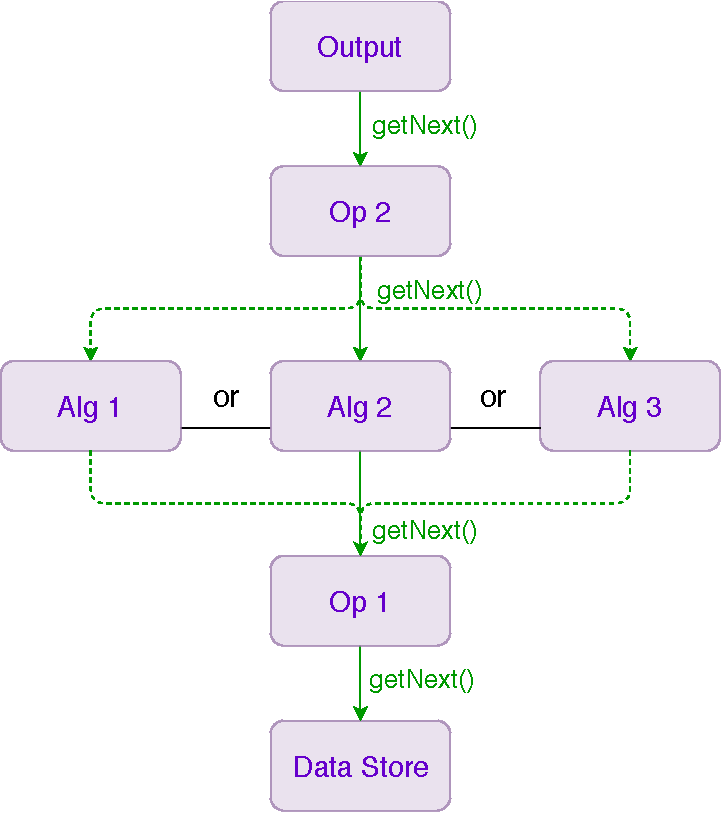
\includegraphics[height=0.6\linewidth]{figures/volcano-model}
	\caption{Query Pipelining with Volcano Model}
	\label{fig:volcano-model}
\end{figure}

% produce/consume
\subsection{Produce/Consume}
The produce/consume concept is slightly different. Each of the database operators has one child operator and one parent operator. All operators implement the common \textit{operator} interface, and thus all possess a child, a parent, as well as the two functions \textit{produce} and \textit{consume}. Whenever an operator needs its child to produce tuples, it calls \textit{produce} on the child. This only happens once, and therefore prevents the operator from continuously calling \textit{next} as it is the case in the Volcano model. After the child received the produce instruction, it first calls \textit{produce} on its own child. As soon as all the tuples have been received and processed, the child repeatedly calls \textit{consume} on its parent and ``feeds'' the tuples to it one by one. The entire process is shown in Fig.~\ref{fig:produce-consume-model}. %There are only as many \textit{consume()} calls as there are tuples to transfer between every two operators. The produce/consume concept, however, is only used during code generation and does not exist at runtime. Just like the volcano model, produce/consume also allows for an easy exchangeability of operators and algorithms, as these can be easily integrated into the query evaluation pipeline \cite{produce-consume}. %TODO: Leave this out?

\begin{figure}[h]
	\centering
	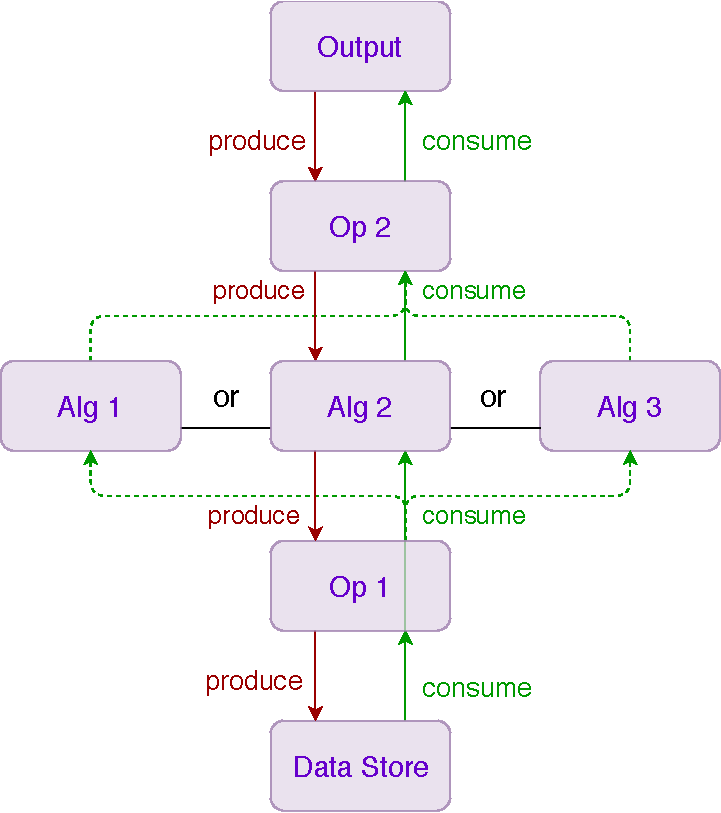
\includegraphics[height=0.6\linewidth]{figures/produce-consume-model}
	\caption{Query Pipelining with Produce/Consume Model}
	\label{fig:produce-consume-model}
\end{figure}

It is important to notice that the produce/consume concept used in this work does \textbf{not} include code generation. Instead, the concept is used ``as-is''. The code is normally compiled and still exists at runtime. A pseudo-code implementation of the produce/consume concept is shown in Algorithm \ref{alg:db-integration}. It features an integration of a sample skyline algorithm into a database system. 

% Pseudocode Integration into DB System with Produce/Consume
\begin{algorithm}[h!]
	\caption{Integration of a Skyline Operator into a Database System} \label{alg:db-integration}
	\begin{algorithmic}[]
		\State \textbf{Input :} Parent Operator $parent$, Child Operator $child$
		%\State \textbf{Output :} Skyline $skyline$
		\State $T \gets New$ List()
		\Function {consume} {Tuple $t$}
			\State Add $t$ to $T$
		\EndFunction
		\Function {produce} {}
			\State $child$.produce()
			\State computeSkyline()
		\EndFunction
		\Function {computeSkyline} {}
			\For {each tuple $t~\in~T$}
				\If {$t$ is not dominated}
					\State $parent$.consume($t$)
				\EndIf
			\EndFor
		\EndFunction
	\end{algorithmic}
\end{algorithm}

% Approaches / frameworks
\subsection{Parallelization Frameworks}
The two main parallelization frameworks utilized in this work are Intel TBB's \textit{parallel\_for}~\cite{parallel-for} construct for C++, as well as the C++ \textit{std::future} library. While the OpenMP~\cite{openmp} API is frequently listed as the main alternative to parallel\_for, the latter seemed slightly more suitable for the purposes of this paper. 

\section{Naive-Nested-Loops and Block-Nested-Loops}
% approach - parallel_for
The main idea when parallelizing the Naive-Nested-Loops algorithm is to use the \textit{parallel\_for} construct for the outer loop of the algorithm. The inner loop could also be taken for this purpose, but then the code which finds itself in the outer loop but not in the inner would be running sequentially, thus reducing the % ``bang for the buck lol''
benefit of parallelizing the code in the first place. 

% pseudo-code parallel NNL
\begin{algorithm}[h]
	\caption{Parallelized Naive-Nested-Loops Algorithm} \label{alg:parallel-nnl}
	\begin{algorithmic}[1]		
		\State \textbf{Input :} Tuple List $T$
		\State \textbf{Output :} Skyline $skyline$
		\PFor {each tuple $t~\in~T$ with \textbf{captured} $T$, $skyline$, $dominates()$}
			\State $is\_not\_dominated \gets $True
			\For {each tuple $d~\in~T\backslash\{t\}$ \textbf{and} as long as $is\_not\_dominated$}
				\If {dominates($d$, $t$)}
					\State $is\_not\_dominated \gets $False
				\EndIf
			\EndFor
			\If {$is\_not\_dominated$}
				\State Add $t$ to $skyline$
			\EndIf
		\EndPFor
	\end{algorithmic}
\end{algorithm}

% implementation
The pseudo-code notation of the parallelized version of Naive-Nested-Loops is given in Algorithm \ref{alg:parallel-nnl}. As global variables and helper functions within the same class, such as $dominates()$ and $T$, cannot by default be ``seen'' from inside the parallelized loop, they are captured and handed over to \textit{parallel\_for} (line 3). The code within the outer loop works similarly to the sequential version, but with one difference. 
The command \textit{Exit inner loop}\footnote{In C++ this is a \textbf{\textit{break}} statement.}, which was previously used in the sequential version of the algorithm (Algorithm \ref{alg:nnl}), is no longer available within a \textit{parallel\_for} loop. This is because it can be problematic for all the threads to coordinate their actions to such an extent that they can all simultaneously break their execution without causing any problems. Therefore, \textit{parallel\_for} does not allow \textit{break} statements. The command has been replaced with the \textit{is\_not\_dominated} flag as a stopping condition in the inner loop (line 5). The algorithm stops as soon as all threads finished their work and eligible tuples find themselves in the $skyline$. 

%Bnl is not as easily parallelizable as NNL. Tried parallel\_reduce on Volcano variant -- didnt improve the performance. Tried NNL with atomic bitmap -- didnt improve the performance. Hence, only poorly parallelizable. 
Several attempts were made to parallelize the Block-Nested-Loops algorithm in this work. The most promising one was to first modify Naive-Nested-Loops so that it would use an atomic bitmap shared between the threads. This bitmap would act similarly to a  ``gravestone'' and would store the indexes of the tuples that are no longer eligible for the skyline. This way, each of the threads would skip any tuples that were already eliminated by other threads, which would significantly reduce its workload. Because this approach uses Naive-Nested-Loops at its base, it is quite easily parallelizable in contrast to the original BNL algorithm. Unfortunately though, it did not produce the expected improvements in running time in comparison to the sequential BNL algorithm. Therefore, no separate parallelized version of BNL is used in the Evaluation chapter (\ref{chapter:Evaluation}) of this work. Instead, two different variants of BNL, one of them using the Volcano model, the other using the Produce/Consume concept will be part of the Evaluation. 

\section{Divide-and-Conquer}
% approach - 2 x parallel_sort, 2 x future, checking size of current set
Two different parallelization techniques were applied to the Divide-and-Conquer algorithm. The first one is another construct from TBB's \textit{parallel} ``family'' called \textit{parallel\_sort}~\cite{parallel-sort}. %The function's syntax is very similar to that of the \textit{std}'s sorting function \textit{sort}. 
Instead of applying a sequential sorting algorithm, \textit{parallel\_sort} sorts the elements using several worker threads simultaneously and thus produces the result significantly faster than sequential functions for large datasets. \textit{parallel\_sort} is applied in two places within the DNC algorithm: 
\begin{enumerate}
	\item It is used within a separate function whose task is to determine the median of a set of tuples. For this purpose, the tuples are first sorted with \textit{parallel\_sort} according to the given dimension. After that, the median of the dataset is taken as the element finding itself exactly in the middle of the sorted set. 
	\item It is used for determining the minimum of a subset of tuples. This functionality is applied when the tuples of the dataset only have two dimensions. In this case, the skyline can be computed by finding the minimum of the first subset and comparing it to all elements of the second subset. % refer to any pseudo-code here?
\end{enumerate}
The second parallelization technique used in DNC is creating two asynchronous threads for the recursive calls of the \textit{mergeBasic} function. As there are three recursive calls to \textit{mergeBasic} from inside the function, one might be thinking of executing all three of them in parallel. Unfortunately, the third call of \textit{mergeBasic} receives the result of the second one as parameter. Therefore, the third call can only be executed as soon as the second one has been completed. As the two parallelized threads run asynchronously, they are not by default waited for by the rest of the code. Because of this, the \textit{future} library offers the method \textit{get} that can be called on each of the parallel thread instances. The function \textit{get} blocks the execution of the program until the result of the corresponding thread is available. As soon as the thread has finished, the result of its computation is returned by \textit{get} and can be used for further operations. 

\section{SARTS and ST-S}
% approach - parallel_sort when presorting, multiple trees
Parallelizing the ST-S and SARTS algorithms results for both of them in almost identical implementation. This is because the main differences between the two algorithms are hidden within the respective tree structures. As the interfaces of both trees are technically the same, the algorithms were also parallelized with the same approach. 

The main idea is to divide the original dataset into as many partitions as there are threads on the machine. For each of these partitions the skyline of its tuples is computed independently in a separate thread. Every thread receives its own tree structure to store the tuples that are part of the skyline and to perform efficient dominance checks. In other words, the sequential version of SARTS (resp. ST-S) is simultaneously applied to each of the partitions. As soon as the skyline of every partition has been computed, the resulting skylines are merged to produce the final skyline. The skylines of all partitions combined are in the utmost cases much smaller than the original dataset. Therefore, the final merge does not take as much time as computing the entire skyline from scratch. 

% illustration to multiple trees approach and ref to it

In addition to the main parallelization approach, presorting the tuples before the actual algorithm begins also happens in parallel. For this purpose, the same \textit{parallel\_sort} construct is used as in the parallelized version of DNC. As the original dataset tends to be very large in real-world applications, sorting it in parallel leads to a very significant ``efficiency boost''. % any proof to large real-world datasets?

% pseudo-code parallel SARTS (essentially the same as parallel ST-S)
The pseudo-code to the parallelized version of SARTS/ST-S is given in Algorithm \ref{alg:parallel-sarts}. 
\begin{algorithm}[h]
	\caption{Parallelized SARTS/ST-S Algorithm} \label{alg:parallel-sarts}
	\begin{algorithmic}[1]		
		\State \textbf{Input :} Number of Threads $n\_threads$, Tuple List $T$, Tree $tree$, Subset Results $sub\_results$
		\State \textbf{Output :} Skyline $skyline$
		\State $subtrees \gets$ undefined
		\For {each $i~\in~N_{0}$, $i~<~n\_threads$}
			\State $subtrees[i]~=$ \textbf{new} Tree()
		\EndFor
		\State $subsets \gets$ undefined
		\For {each $i~\in~N_{0}$, $i~<~n\_threads$}
			\State $subsets[i] \gets T[i~*~T.size~/~n\_threads]$ until $T[(i~+~1)~*~T.size~/~n\_threads~-~1]$
			\State Start \textbf{new} asynchronous Thread() for compute\_skyline\_subset($i$, $subsets[i]$, $subtrees[i]$)
		\EndFor	
		\For {each asynchronous Thread $t$}
			\State Wait for $t$ to finish
		\EndFor		
		\State $skyline \gets$ Skyline($sub\_results$, $tree$) $~~~~~$ {\footnotesize // Compute Skyline either with SARTS or ST-S}
		
%		\State Sort tuples in $sub\_results$ in-place using a monotonic function \textit{minC()}
%		\State $t_{0} \gets $ first element of $sub\_results$
%		\State $t_{stop} \gets t_{0}$
%		\State insert($t_{0}$, $tree.root$, 0)
%		\State Add $t_{0}$ to $skyline$
%		\For {each tuple $t~\in~sub\_results\backslash\{t_{0}\}$}
%			\If {$max$($t_{stop}$)$~\leq~min$($t$) and $t_{stop}~\neq~t$}
%				\textbf{return}
%			\EndIf
%			\If {\textbf{not} is\_dominated($t$, $tree.root$, 0, $score(t)$)}
%				\State insert($t$, $tree.root$, 0)
%				\State Add $t$ to $skyline$
%				\If {$max(t)~<~max(t_{stop})$}
%					\State $t_{stop} \gets t$ 
%				\EndIf
%			\EndIf
%		\EndFor	
		
	\end{algorithmic}
\end{algorithm}
% algorithm description
\begin{enumerate}
	\item At first, the tree structures $subtrees$ are initialized for each of the threads to run in parallel on their subset of tuples (lines 3-5).
	\item Then, the subsets are filled with the respective range of tuples from the original dataset (lines 7-8). In the given pseudo-code, the dataset is simply partitioned into sequential ranges of equal size. There are exactly as many partitions as there are threads. 
	\item For each of the subsets, a new asynchronous thread is started and receives its thread ID, the corresponding subset and an empty tree, for instance ART, as parameters (line 9). 
	\item After all the threads have been started, they compute their sub-skylines in parallel and store the resulting candidate tuples into a common array called $sub\_results$. 
	\item As soon as the threads have finished their work (lines 10-11), their results are merged into the final skyline. This is done by applying the sequential version of SARTS/ST-S as presented in chapter \ref{section:sarts} (resp. \ref{subsection:sts} for ST-S) to $sub\_results$. 
\end{enumerate}

The pseudo-code to the \textit{compute\_skyline\_subset} operation for parallelized SARTS/ST-S is given in Algorithm \ref{alg:parallel-sarts-subskyline}. 
\begin{algorithm}[h]
	\caption{COMPUTE\_SKYLINE\_SUBSET for Parallelized SARTS/ST-S} \label{alg:parallel-sarts-subskyline}
	\begin{algorithmic}[1]		
		\State \textbf{Input :} Thread Number $tid$, Number of Threads $n\_threads$, Tuple Subset $T$, Tree $sub\_tree$, Subset Results $sub\_results$
		\State Sort $ T $ in-place using a monotonic function \textit{minC()}
		\State $t_{0} \gets $ first element of $T$
		\State $t_{stop} \gets t_{0}$
		\State insert($t_{0}$, $sub\_tree.root$, 0)
		\State Add $t_{0}$ to $sub\_results$ at position $tid~*~(sub\_results.size~/~n\_threads)$
		\For {each tuple $t~\in~T\backslash\{t_{0}\}$}
			\If {$max$($t_{stop}$)$~\leq~min$($t$) and $t_{stop}~\neq~t$}
				\textbf{return}
			\EndIf
			\If {\textbf{not} is\_dominated($t$, $sub\_tree.root$, 0, $score(t)$)}
				\State insert($t$, $sub\_tree.root$, 0)
				\State Add $t$ to $sub\_results$ at position $tid~*~(sub\_results.size~/~n\_threads)~+~t.index$
				\If {$max(t)~<~max(t_{stop})$}
					\State $t_{stop} \gets t$ 
				\EndIf
			\EndIf
		\EndFor		
	\end{algorithmic}
\end{algorithm}

% algorithm description
Instead of computing the skyline on the entire set of tuples, the function only takes a subset of the original data as argument. It also receives the ID of the thread that it is assigned to, the overall number of threads running in parallel, as well as a reference to an array where the skyline results of all subsets will be stored. 

The skyline is computed similarly to the non-parallelized version with one major difference. Whenever a tuple that is definitely part of the skyline is stored, it is not just appended to some list of skyline tuples. Instead, it is stored into the common $sub\_results$ array which all skyline threads share access to. In order to prevent any sort of race condition during \textit{write} operations between the threads, each of the threads writes its results strictly into the part of the array assigned to this particular thread (lines 6, 11). %The starting index of the correct writing range for one thread is determined by multiplying this thread's number with the size of the array divided by the whole number of threads (lines 6, 11). The correct position for a candidate tuple within the array is determined by simply adding its index in the subset to the range's starting point (line 11). 







